\documentclass[12pt, a4paper]{third-rep}

% go fast
% \def\compileFast{a}

% colours
\usepackage{xcolor}
\definecolor{mydarkblue}{rgb}{0,0.08,0.45}
\definecolor{mintbg}{rgb}{0.95,0.95,0.95}
\definecolor{listingframe}{rgb}{1,0.31,0}

% tcolorbox my beloved
\usepackage{tcolorbox}
\tcbuselibrary{skins,listings,raster,minted,breakable}
\newtcbinputlisting[auto counter]{\pythoncode}[3][]{
  enhanced jigsaw,breakable,
  boxrule=0.2mm,top=1mm,bottom=1mm,left=1mm,right=1mm,
  before=\par\smallskip,after=\par\smallskip,
  listing file={#3},
  listing only,
  listing engine=minted,
  listing options={basicstyle=\footnotesize\listingsfont},
  minted language=python,
  minted style=colorful,
  colback=mintbg,
  colframe=listingframe,
  fonttitle=\bfseries,
  title={Listing \thetcbcounter: #2},
  #1
}

% graphics
\usepackage{graphicx}
\graphicspath{ {assets/} }

% minted replaces listings
\usepackage{minted}
\usepackage{dingbat}
\setminted[python]{
    breaklines,
    breakanywhere,
    autogobble,
}

% hyperlink setup
\usepackage{url}
\usepackage{hyperref}
\hypersetup{
    pdftitle={},
    pdfsubject={},
    pdfkeywords={},
    pdfborder=0 0 0,
    pdfpagemode=UseNone,
    colorlinks=true,
    linkcolor=mydarkblue,
    citecolor=mydarkblue,
    filecolor=mydarkblue,
    urlcolor=mydarkblue,
}

% used for nesting figures
\usepackage{subcaption}

% Maths/CS symbols
\usepackage{stmaryrd}
\usepackage{amsmath}
\usepackage{amssymb}
\usepackage{amsfonts}

% cleverly decides how to reference a given ref
% must be loaded after hyperref and amsmath
\usepackage{cleveref}

% cite things with a small superscript number
\usepackage[superscript,biblabel]{cite}

% package for defining custom math symbols
\usepackage{stackengine}
\stackMath
\newcommand{\cryptoSample}{\shortleftarrow\kern-1.5ex\text{\scriptsize \$}}

%% Uncomment the following lines if you want to include the date as a
%% header in draft versions. See the documentation for fancyhdr for
%% more ways of modifying headers (texdoc fancyhdr will show you the
%% docs) 

% \usepackage{fancyhdr}
% \setlength{\headheight}{14.5pt} % silence warnings
% \pagestyle{fancy}
% \lhead{}  % left head
% \chead{Draft: \today} % centre head
% \lfoot{}
% \cfoot{\thepage}
% \rfoot{}

% title stuff
\usepackage{titlesec}
\newcommand{\PreContentTitleFormat}{\titleformat{\chapter}[display]{\scshape\Large}
{\Large\filleft\MakeUppercase{\chaptertitlename} \Huge\thechapter}
{1ex}
{}
[\vspace{1ex}\titlerule]}

\newcommand{\ContentTitleFormat}{\titleformat{\chapter}[display]{\scshape\huge}
{\Large\filleft\MakeUppercase{\chaptertitlename} \Huge\thechapter}
{1ex}
{\titlerule\vspace{1ex}\filright}
[\vspace{1ex}\titlerule]}

% glossary stuff
\usepackage[toc]{glossaries}
\setacronymstyle{long-short}
\makenoidxglossaries{}
\loadglsentries{glossary}

% Tikz stuff
\usepackage{tikz}
\ifx\compileFast\undefined
  \usepackage{tikzpeople}
\else
  \usepackage[draft]{tikzpeople}
\fi

% plotting things
\usepackage{pgfplots}
\pgfplotsset{compat=1.18}
\usetikzlibrary{intersections,decorations.markings}

\newcommand{\plotcurve}[3][thick, every plot/.style={smooth}]{
  % plot curve y^2 = x^3 + a x + b in range [-3,3]^2
  % parameter 1 (optional): style options for curve (color, etc)
  % parameter 2: curve parameter a
  % parameter 3: curve parameter b
  \draw[gray] (-3,-3) rectangle (3,3);
  \draw[->,>=latex,gray] (-3,0) -- (3,0);
  \draw[->,>=latex,gray] (0,-3) -- (0,3);
  \draw[name path=curve, #1] plot[id=curve#2#3, raw gnuplot] function {
    f(x,y) = y**2 - x**3 - #2*x - #3;
    set xrange [-3:3];
    set yrange [-3:3];
    set view 0,0;
    set isosample 50,50;
    set cont base;
    set cntrparam levels incre 0,0.1,0;
    unset surface;
    splot f(x,y);
  };
}

\tikzset{
  tangent/.style={
    decoration={markings, mark=at position #1 with {
      \coordinate (tangent point-\pgfkeysvalueof{/pgf/decoration/mark info/sequence number}) at (0pt,0pt);
      \coordinate (tangent unit vector-\pgfkeysvalueof{/pgf/decoration/mark info/sequence number}) at (1,0pt);
      \coordinate (tangent orthogonal unit vector-\pgfkeysvalueof{/pgf/decoration/mark info/sequence number}) at (0pt,1);
    }},
    postaction=decorate
  },
  use tangent/.style={
    shift=(tangent point-#1),
    x=(tangent unit vector-#1),
    y=(tangent orthogonal unit vector-#1)
  },
  use tangent/.default=1
}

% crypgraphy stuff
\usepackage[operators, sets]{cryptocode}

% only work on a chapter at a time to improve compile times
\ifx\compileFast\undefined
\else
  \includeonly{chapter1,appendix1,appendix2}
\fi

\title{Exploring Password-Authenticated Key-Exchange Algorithms}
\author{Sam Leonard}
\supervisor{Professor Bernardo Magri}
\reportyear{2023}
\studentid{f41751sl}

\abstractfile{abstract.tex}
\thanksfile{merci.tex}

\begin{document}

\dotitleandabstract

%% Generate contents etc
\tableofcontents

%% These include the actual text
\chapter{Introduction}
\label{chap:intro}

Today's standards for Encryption and Authentication are fundamentally broken.
The age old standard practice of obtaining an encrypted connection to a server, then sending a cleartext password to authenticate users is flawed.
\glspl{pake} are a profoundly different way of looking at how encryption and authentication are performed, and could represent the basis for a safer and more secure future, even in the face of the ever increasing threat quantum computers pose to encryption.

\section{Aims}
This project aims to understand the nature of how \glspl{pake} work, what they can and cannot do, and how they can be used to improve the security of almost all password based authentication systems.
The \enquote{quantum annoying} property of \glspl{pake} will also be explored, to understand how \glspl{pake} can be used to delay the need for post-quantum cryptography by years or even decades \cite{quantum-annoying}.
Additionally an implementation of a modern \gls{pake} protocol (\gls{aucpace}) will be created and and contributed back to the RustCrypto open source project.

\section{Deliverables}
The implementation of the \gls{aucpace} protocol in Rust is the core deliverable for this project.
Performance of the library will be compared against those for other \gls{pake} protocols.
The metrics of execution time, code size and message size will be used.

\section{Challenges}
Working with elliptic curve cryptography proved to be particularly challenging.
A lack of understanding of one particular area proved fatal when a catastrophic bug was found in the codebase late in the project.
\Cref{chap:testing} talks about remediating this bug and ensuring it cannot happen again.

\section{Structure}
The report will follow the following structure:
\begin{itemize}
    \item{\Cref{chap:intro} introduces the project and provides an explanation of the aims and deliverables.}
    \item{\Cref{chap:context} goes into detail on the history of \gls{pake} algorithms and explains elliptic curve cryptography.}
    \item{\Cref{chap:design} explains the design decisions made around the implementation of \gls{aucpace}.}
    \item{\Cref{chap:impl} talks about how the library was implemented, how Rust's type and trait systems were effectively utilised to make the library as easy to use as possible.}
    \item{\Cref{chap:testing} covers the extensive testing of the library, from unit and integration testing to running the protocol on real hardware. A comparison to an equivalent \gls{pake} (\gls{opaque}) is made by benchmarking both libraries. Finally the bug from above is explored, the fix and future prevention are explained.}
    \item{\Cref{chap:conclusion} wraps up the project, with a reflection and an analysis of possible future work.}
\end{itemize}

\chapter{Design}

\section{Why Rust?}
\label{sec:why-rust}

\gls{aucpace} explicitly targets \gls{iiot} in it's design.
Rust is rapidly becoming a popular choice for \gls{iot} and embedded software applications.
This is due to it's focus on memory safety, developer experience and it's strong embedded ecosystem.
Libraries like Embassy and RTIC allow the user to program high level logic and use powerful abstractions to interact with the hardware through Rust objects, while still compiling down to small efficient binaries.
Embassy is especially impressive as they have implemented a async executor so that multitasking in embedded applications can be performed with the same async/await framework that programmers are familiar with.
A short Embassy examples is shown in listing \ref{embassy-example}.
Tools such as \texttt{probe-rs} allow developers to maintain the same workflow they would when working on a normal rust binary, by implementing a \texttt{cargo} runner which flashes the binary to the embedded device then using \gls{rtt} to receive debug messages from the device.
Those debug messages can be setup automatically using libraries such as \texttt{defmt\_rtt} which use \gls{rtt} to send a compressed representation of the debug message to be formatted later on using a technique called deferred formatting, allowing for debug messages to take up a fraction of the size of the original message.

\rustcode[label=embassy-example]{Embassy async/await example}{assets/embassy_example.rs}

\section{Developer Focussed Design}


\chapter{Design}
\label{chap:design}

\section{Why Rust?}
\label{sec:why-rust}

\gls{aucpace} explicitly targets \gls{iiot} in it's design.
Rust is rapidly becoming a popular choice for \gls{iot} and embedded software applications.
This is due to it's focus on memory safety, developer experience and it's strong embedded ecosystem.
Libraries like Embassy and \gls{rtic} allow the user to program high level logic and use powerful abstractions to interact with the hardware through Rust objects, while still compiling down to small and efficient binaries.
Embassy is especially impressive as they have implemented an async executor so that multitasking in embedded applications can be performed with the same async/await framework that programmers are familiar with.
A short Embassy examples is shown in listing \ref{embassy-example}.
Tools such as \texttt{probe-rs} allow developers to maintain the same workflow they would when working on a normal Rust binary, by implementing a \texttt{cargo}\footnote{cargo is the standard build system for Rust.} runner which flashes the binary to the embedded device then uses \gls{rtt} to receive debug messages from the device.
Those debug messages can be setup automatically using libraries such as \texttt{defmt\_rtt} which use \gls{rtt} to send a compressed representation of the debug message to be formatted later on using a technique called deferred formatting, allowing for debug messages to take up a fraction of the size of the original message.
Together this makes Rust a compelling choice for writing embedded code.

\medskip{}

\rustcode[label=embassy-example]{Embassy async/await example}{assets/embassy_example.rs}

Rust is also very well suited for implementing cryptographic software.
It's lifetimes system and compile time safety guarantees make it ideal for building security focused software.
Rust was recently added to \gls{nist}'s list of \enquote{Safer Languages} which it recommends for writing safety focused programs in \cite{nist-safer-languages}.

As well as this many algorithms, formats and primitives are implemented, and freely available as crates\footnote{\enquote{crates} in Rust are code libraries which are publically available for anyone to use via cargo -- the Rust toolchain} for anyone to use.
Rust's trait system also lends itself well to this, it is possible to use implement a trait representing an elliptic curve and then an algorithm can be written to be agnostic about the curve that it is using for instance.
This allows library writers to easily write generic code to give user's of the libraries as much flexibility and choice around how they implement their program.
This is especially important for systems which might need to interact with legacy systems or that need to provide a certain level of security for \gls{fips} standards like \gls{fips}-140-2 \cite{fips-140-2}.

\section{Planning the Library}
Before implementing \gls{aucpace} it was necessary to plan ahead what libraries to use.
Without planning it would be easy to end up in a situation where different libraries aren't compatible with each other, or have become superseded by another library as this information is not readily available on \href{https://crates.io/}{crates.io} (crates.io is the package repository for all public Rust packages).

\subsection{What Primitives Do We Need To Implement AuCPace?}
\gls{aucpace} has many parameters which can be changed to drastically change how the protocol works, this is by design to allow customisability for each user's needs, however it can be quite confusing to navigate.
As such it is worthwhile to look at the parameters are and thus what primitives we will need.
\Cref{tab:aucpace-params,tab:aucpace-selected-params} are partially reproduced from \cite{aucpace} just in significantly fewer words.

\begin{center}
  \rowcolors{0}{}{mintbg}
  \captionof{table}{\gls{aucpace} Parameters}
  \label{tab:aucpace-params}
  \begin{tabularx}{\linewidth}{ cX }
    \toprule
    parameter & explanation \\
    \midrule
    $\textsf{PBKDF}_{\sigma}$ & A \gls{pbkdf} parameterised by $\sigma$.
    The parameters of the \gls{pbkdf} are algorithm specific, but usually would include settings such as the memory consumption of the algorithm, the hash used or the iteration count (number of times to perform the hash). \\
    $\mathcal{C}, \mathcal{J}, c_{\mathcal{J}}, B$ & A (hyper-)elliptic curve $\mathcal{C}$ with a group $\mathcal{J}$ with co-factor $c_{\mathcal{J}}$ and a \gls{dh} protocol operating on both, $\mathcal{C}$ and it's quadratic twist $\mathcal{C}'$. $B$ denotes the \gls{dh} base point in $\mathcal{J}$.\\
    \textsf{Map2Point} & A function mapping a string $s$ to a point from a cryptographically large subgroup $\mathcal{J}_m$ of $\mathcal{C}$. The inverse map $\textsf{Map2Point}^{-1}$ is also required.\\
    $\textsf{H}_0 \dots \textsf{H}_5$ & A set of 6 distinct hash functions.\\
    \bottomrule
  \end{tabularx}
\end{center}

\begin{center}
  \rowcolors{0}{}{mintbg}
  \captionof{table}{Selected parameters of the reference implementation -- AuCPace25519}
  \label{tab:aucpace-selected-params}
  \begin{tabularx}{\linewidth}{ cX }
    \toprule
    parameter & explanation \\
    \midrule
    $\textsf{PBKDF}_{\sigma}$ & Scrypt \cite{scrypt} an optimally memory-hard \cite{scrypt-max-mem-hard} \gls{pbkdf}, parameterised with a memory usage of 32Mb.\\
    $\mathcal{C}, \mathcal{J}, c_{\mathcal{J}}, B$ & Curve25519 \cite{curve25519} a Montgomery form elliptic curve, with excellent speed properties.
      X25519 an x-coordinate-only \gls{dh} protocol.\\
    \textsf{Map2Point} & The Elligator2 map introduced by \citeauthor{elligator2} in \cite{elligator2}.\\
    $\textsf{H}_0 \dots \textsf{H}_5$ & The \glslink{sha}{SHA512} hash function where the index is prepended as a little-endian four-byte word.\\
    \bottomrule
  \end{tabularx}
\end{center}

So in summary we need the following primitives:
\begin{itemize}
  \item{a \gls{pbkdf}}
  \item{an elliptic curve, a group on the curve, a \gls{dh} protocol operating on the group}
  \item{a mapping from strings to curve points}
  \item{a hash function}
\end{itemize}

\subsection{What Rust Libraries Actually Exist For Cryptography?}
There are many sites online which act as collections of Rust packages that you can search by topic to find similar or related packages.
The \gls{rcig} maintain a list of Rust's Cryptographic libraries at \url{https://cryptography.rs/}, this proved to be a great help while researching libraries.

For the required primitives the following Rust crates were identified as potential candidates:
\begin{itemize}
  \item{
    The \gls{pbkdf}:
    \begin{itemize}
      \item{\href{https://github.com/RustCrypto/password-hashes/tree/master/argon2}{\texttt{argon2}} -- RustCrypto's Argon2 implementation}
      \item{\href{https://github.com/RustCrypto/password-hashes/tree/master/pbkdf2}{\texttt{pbkdf2}} -- RustCrypto's PBKDF2 implementation}
      \item{\href{https://github.com/RustCrypto/password-hashes/tree/master/scrypt}{\texttt{scrypt}} -- RustCrypto's Scrypt implementation}
      \item{\href{https://github.com/Keats/rust-bcrypt}{\texttt{rust-bcrypt}} -- a pure Rust Bcrypt implementation}
      \item{\href{https://github.com/sru-systems/rust-argon2}{\texttt{rust-argon2}} -- a pure Rust Argon2 implementation}
      \item{\href{https://github.com/RustCrypto/traits/tree/master/password-hash}{password-hash} -- trait to allow implementations to be generic over the password hashing algorithm used}
    \end{itemize}
  }

  \item{
    The elliptic curve:
    \begin{itemize}
      \item{\href{https://github.com/dalek-cryptography/curve25519-dalek}{\texttt{curve25519-dalek}} -- Dalek Cryptography's implementation of Curve25519 and Ristretto255 \cite{ristretto255}}
      \item{\href{https://github.com/RustCrypto/traits/tree/master/elliptic-curve}{\texttt{elliptic-curve}} -- traits for operating over a generic elliptic curve, part of RustCrypto}
      \item{\href{https://github.com/RustCrypto/elliptic-curves}{\texttt{elliptic-curves}} -- RustCrypto's meta-repo holding implementations for the following curves: brainpoolP256r1/t1, brainpoolP384r1/t1, Secp256k1, P-224, P-256, P-384, P-521}
    \end{itemize}
  }

  \item{
    The \textsf{Map2Point} function:
    \begin{itemize}
      \item{\href{https://github.com/dalek-cryptography/curve25519-dalek}{\texttt{curve25519-dalek}} -- includes \verb|RistrettoPoint::from_uniform_bytes| which implements Ristretto flavoured Elligator2}
      \item{\href{https://github.com/RustCrypto/traits/tree/master/elliptic-curve}{\texttt{elliptic-curve}} -- includes \texttt{MapToCurve} which implements the hash-to-curve operation for NIST P-256 and Secp256k1}
    \end{itemize}
  }

  \item{
    The hash function:
    \begin{itemize}
      \item{\href{https://github.com/RustCrypto/traits/tree/master/digest}{\texttt{digest}} -- a trait for operating generically over hash functions, from RustCrypto}
      \item{\href{https://github.com/RustCrypto/hashes}{\texttt{hashes}} -- RustCrypto's meta-repo holding implementations for the following hashes: Ascon, BLAKE2. KangarooTwelve, SHA2, SHA3, Tiger, Whirlpool, and several more.}
    \end{itemize}
  }
\end{itemize}

\subsection{Picking Crates for the Required Primitives}
Where possible the implementation should match the reference implementation.
These choices are what the designers have determined as secure presets so they are good choices should a suitable crate exist.

\subsubsection{Choosing the PBKDF}
Instead of picking a \gls{pbkdf} up front, the \texttt{PasswordHasher} trait from \href{https://github.com/RustCrypto/traits/tree/master/password-hash}{password-hash} allows us to be generic over the \gls{pbkdf} when implementing the library.
Allowing users of the library to pick from either Argon2, Scrypt or PBKDF2 at their discretion, or to implement their own algorithm and supply an implementation of \texttt{PasswordHasher} for it.

\subsubsection{Choosing the Curve and \textsf{Map2Point} Operation}
Although the \texttt{elliptic-curves} repo implements many different elliptic curves, it doesn't implement Curve25519\footnote{there is currently a push to have it included in the crate, though it is still early on and the implementation is not fit for use}, and the \texttt{hash2curve} \gls{api} for \gls{nist} P-256 uses the \gls{osswu} map \cite{osswu-map}, which is known to be less efficient than the Elligator2 map defined for Montgomery curves \cite{elligator2}.
There have also been questions about whether the coefficients used in \gls{nist}'s suite of curves have been deliberately tampered with \cite{curve-rigidity}.

Another issue to consider when picking a curve and group is the problem of cofactor handling.
To avoid mishandling group cofactors \gls{aucpace} shows everywhere a cofactor multiplication is necessary, failing to perform one of these multiplications would be a serious bug.
However we can eliminate the need for handling cofactors altogether by using a prime order group, that is a group with a prime number of elements in it.
Ristretto255 \cite{ristretto255} is one such group built on top of Curve25519.
The \texttt{curve25519-dalek} crate implements Ristretto255 as well as the Ristretto flavoured Elligator2 map \cite{elligator2} which implements the required \textsf{Map2Point} operation.

\subsubsection{Choosing the Hash Function}
The hash function is another parameter that is easy to be generic over, thanks to the \texttt{digest} crate.
This allows users to pick from the plethora of hashes implemented by \texttt{RustCrypto/hashes}, enabling them to choose whichever hash function is best suited for their application.

\section{Initial Designs for the Structure of the Library}
Rust is very flexible in regards to how you wish to structure a library, there are many patterns that are known to work well in Rust and as such have become Rust idioms.
Rust is fairly unique among programming languages as it offers very little in the way of inheritance, unlike classes in Java or C++, Rust's structs cannot inherit from each other.
Instead if you want to implement some functionality on top of another type you must in some way store a value of that type.
As such wrapper structs are common in Rust, the most common use of these would be the iterator adapters.
The \texttt{Iterator} trait from the standard library has many methods for providing common operations which are agnostic to what is being iterated over, e.g. \texttt{Iterator::filter}, \texttt{Iterator::map} and \texttt{Iterator::rev}.
Each of these methods returns a specialised struct which contains the initial iterator, specifically \texttt{std::iter::Filter}, \texttt{std::iter::Map} and \texttt{std::iter::Rev} for the aforementioned methods.
These structs are all \textit{owning}, meaning they own the data they contain.
The concept of Ownership is central to Rust, it forms the basis for how the borrow checker works and is the main mechanism by which Rust can guarantee memory safety.
In general owned types are always easier to work with than borrowed ones, you don't have to keep track of lifetimes and in general life is easier.
The main use-case for references is for when you have some value that you either cannot copy, (e.g. a Mutex), or really don't want to copy (e.g. 10Gb worth of data).

This preference for Owned values leads to one slightly messy but easy to implement pattern whereby one struct is used to implement all of the functionality and all of the state is bundled in this one struct.
While easy to implement this approach does have some drawbacks, some of the state might only be needed for one operation then it is worthless, however having everything in one struct means that the space is still allocated whether you need it or not.
Being aware of this is especially pertinent as the amount of state required gets larger.

\subsection{There Are Other PAKEs Implemented in Rust, How Are They Designed?}
RustCrypto have implemented two \glspl{pake} -- \gls{srp} and \glslink{spake}{SPAKE2}.
\glslink{spake}{SPAKE2} is the simpler of the two protocols so lets analyse it first.

\subsubsection{Exploring RustCrypto's SPAKE2 Implementation}
A diagram of the \glslink{spake}{SPAKE2} protocol can be found in \cref{fig:spake2}.
The core of the implementation is the following struct:
\rustcode{SPAKE2 Struct}{assets/spake2.rs}

It contains an owned copy of every piece of data needed to run the entire protocol, although there are quite a few members here, \glslink{spake}{SPAKE2} effectively requires it as the final key $SK_B$ is calculated as $H(A, B, X^*, Y^*, Kb)$, in addition this is a very simple protocol at only one message each way.
This means that there isn't as much overhead for keeping lots of data around.

The \gls{api} exposed by the struct is also very simple, there are number of \texttt{start\_*} methods which begin the protocol and generate initial values from the \gls{csprng}, all of these methods return a tuple \texttt{(<state>, <message>)}.
The message can then be sent to the other party and when the response is received there is a single \texttt{finish} method which takes in this response and produces a \texttt{Result<Vec<u8>>}\footnote{Rust's Result type is used to return a value or an error, the type system forces handling this value and the code will panic if a value is expected and an error occurs. It is very similar to Haskell's Maybe type.}, this contains the shared key if everything went well and an error otherwise.

In summary it is implemented as one large struct with many helper methods for all the different ways to start the protocol.

\subsubsection{Exploring RustCrypto's SRP Implementation}
A diagram of the \gls{srp} protocol can be found in \cref{fig:srp}.

As \gls{srp} is an \gls{apake} it is implemented with a separate \texttt{Client} and \texttt{Server} struct as seen below.

\rustcode{SRP Server Struct}{assets/srp_server.rs}
\rustcode{SRP Client Struct}{assets/srp_client.rs}

However it is plain to see these structs hold the same values, the only difference is the methods available on each.
This is a completely different approach to the \glslink{spake}{SPAKE2} library.
In this design how the state is stored is left entirely up to the library consumer, with these structs simply implementing all of the methods for the computation at each step.
This does expose a very flexible API and store the absolute minimum amount of data, however it doesn't do anything to protect from accidental misuse by the programmer.

\subsection{Initial Design Plan}
To support contributing the implementation back to RustCrypto, the library will be implemented as a fork of \url{https://github.com/RustCrypto/PAKEs},
where the \gls{aucpace} implementation will be added as a new crate in the Cargo workspace.

As a prototype for the library functionality a design in the style of RustCrypto's \gls{srp} implementation was created to explore how the computations required by \gls{aucpace} look in Rust and how the different libraries interact together.

After this prototype version several attempts were made at a more user-friendly / intuitive design, eventually settling on one where the user \enquote{moves} between various structs by passing messages between the server and client.
Each move returns either just the next state, or a tuple of a message and the next state, it is then the user's job to manage just the communication of messages between the client and server.
This approach reduces the cognitive overhead of the developer and allows them to just focus on the core of a protocol -- passing messages.


\chapter{Implementation}
\label{chap:impl}

\section{Creating the initial prototype}
The initial prototype was based around the \gls{srp} implementation from RustCrypto.

\rustcode{AuCPace Server Prototype}{assets/aucpace_server_prototype.rs}
\rustcode{AuCPace Client Prototype}{assets/aucpace_client_prototype.rs}

This struct then implemented methods for each of the computations needed by the protocol.

\section{Adding feature flags}
\section{Adding Partial Augmentation}
\section{Adding Partial Augmentation}

\chapter{Testing}
\label{chap:testing}

\section{Testing for correctness of functionality}
As the library is built on other crates, the only tests which can be performed are those on individual components of the protocol, and full run-throughs of the entire protocol.

\subsection{Testing individual components}
Traditionally in cryptographic software, test-vectors have been used to test for the correct functionality of various componenets.
However due to the use of Ristretto255, instead of raw Curve25519, there are no test-vectors available.
Once the implementation was feature complete, I emailed Bj\"orn Haase to discuss test vector creation\footnote{Bj\"orn is the creator of AuCPace}.
He was interested in the project and mentioned they were interesteed in a second implementation of \gls{aucpace} at Endress+Hauser.
However he did not have the time to create test vectors and by this point in the project I was too busy to do so as well.
So while test vectors have not yet been created, it is likely they will be in the near future.

\subsection{Integration testing}
To perform integration testing, the tests were split into four categories based on which of the two major features they required\footnote{This work was completed after the code freeze, so is only available on the github.}.

\begin{center}
  \rowcolors{0}{}{mintbg}
  \captionof{table}{Integration Tests Split}
  \label{tab:aucpace-int-tests}
  \begin{tabularx}{\linewidth}{ ccX }
    \toprule
    \texttt{strong\_aucpace} & \texttt{partial\_aug} & test \\
    \midrule
    \xmark & \xmark & \texttt{test\_key\_agreement.rs} \\
    \xmark & \cmark & \texttt{test\_key\_agreement\_partial\_aug.rs} \\
    \cmark & \xmark & \texttt{test\_key\_agreement\_strong.rs} \\
    \cmark & \cmark & \texttt{test\_key\_agreement\_strong\_partial\_aug.rs} \\
    \bottomrule
  \end{tabularx}
\end{center}

Inside of each test file there are two main scaffolding functions: \texttt{init} and \texttt{test\_core}, the former Perfoms the initial setup of the client, server and database, and the latter performs all the functionality which is common to every test.
From there there are four tests in each file, each testing the following:

\begin{center}
  \rowcolors{0}{}{mintbg}
  \captionof{table}{Per-file Test Splits}
  \label{tab:aucpace-int-tests-file}
  \begin{tabularx}{\linewidth}{ ccX }
    \toprule
    \texttt{static SSID} & \texttt{implicit auth} & test \\
    \midrule
    \xmark & \xmark & \texttt{test\_key\_agreement} \\
    \xmark & \cmark & \texttt{test\_key\_agreement\_implicit\_auth} \\
    \cmark & \xmark & \texttt{test\_key\_agreement\_prestablished\_ssid} \\
    \cmark & \cmark & \texttt{test\_key\_agreement\_prestablished\_ssid\_implicit} \newline \texttt{\_auth} \\
    \bottomrule
  \end{tabularx}
\end{center}

\section{The Ultimate Test}
As with any piece of software the ultimate test is to get the entire thing running / working on real hardware.

\subsection{Choosing the Microcontroller / Platform}
Because \gls{aucpace} is intended for use in the \gls{iiot}, it was decided that an \gls{stm} based \gls{mcu} would be a good fit.
\gls{stm} \glspl{mcu} are very prevelant in industry, have many dev boards supporting a wide variety of different chips, and they also have excellent rust support.
Following this decision the NUCLEO-F401RE dev board was selected.
It is a small \gls{mcu} with a modest 512K of flash memory.
While certainly not the least powerful platform around it should be representative of a majority of \gls{iot} systems.

\begin{figure}[H]
  \centering

  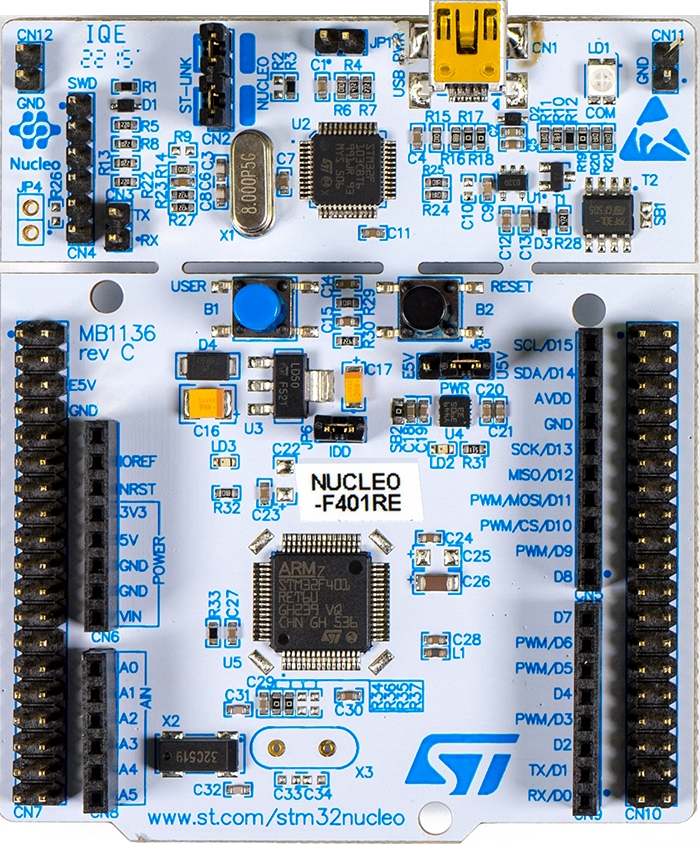
\includegraphics[angle=90,width=0.8\linewidth]{assets/stm32-f410re.jpg}
  \caption{NUCLEO-F401RE Dev Board}
  \label{fig:nucleo-f401re}
\end{figure}

\subsection{Choosing an Embedded Rust Platform}
Initially the \gls{rtic} framework was selected as example code for interacting over serial was easy to find online.
However getting \gls{rtic} to work on the actual board proved challenging as low level details such as clocks and timers confused things considerably.

After a few attempts\footnote{several days of work} with \gls{rtic}, efforts were switched to using the Embassy project.
This proved to greatly alleviate the strain of working in the embedded software world.
Embassy performs all low level setup for you and allows the programmer to work with async/await constructs instead of timers etc.
There was still some considerable strife in getting the serial connection to work consistently.
After a lengthy conversation with \texttt{sjm\#0205} on the Rust discord server, we came to the conclusion that the board's low quality crystal oscillators were causing the serial connection to get out of sync.
Reducing the baud rate to 28800 resulted in a much more reliable connection, this is due to clock accuracy being less important at lower baud rates as there is a bigger margin for error in when lines go high/low\footnote{This solution was found after code freeze so is only available on the github}.
After establishing a reliable serial connection work could now begin on implementing \gls{aucpace}.

\subsection{Implementing the AuCPace protocol}
The server side of \texttt{examples/key\_agreement.rs} was initially adapted to fit the code structure of the embedded app.
However this immediately brought around a problem with the \gls{aucpace} implementation, it was refusing to compile.
As it happened this was a quirk of how rust works that I wasn't aware of.
Care was taken to develop the library using the \verb|#[no_std]| attribute, this tells the compiler that this code isn't allowed to use the Rust standard library.
Even the \texttt{examples/key\_agreement\_no\_std.rs} example program wasn't enough to weed this out.
Because the standard library is still available when linking on x86, the \verb|#[no_std]| example still compiles, despite containing code from the standard library.
When it was adapted for the microcontroller, it was targeting \texttt{thumbv7em-none-eabihf}, the standard library is simply not available for this target as it doesn't have an operating system.
The malignant crate turned out to be \texttt{serde-arrays} which, although not containing any code that should require the standard library, it was not marked as \verb|#[no_std]| and thus fails to compile as it implicitly links to the standard library.
The solution was very simple thankfully, just weeks prior to attmpting this embedded example, a new crate was released \texttt{serde-byte-arrays}, this solved my problem better than \texttt{serde-arrays}, was marked \verb|#[no_std]| and was more efficient at the same time!
Once these two primitives were reliable, it was quite straightforward to implement the protocol in full.

% mention hitting NLL problem case 3?

\subsection{benchmarking}
Benchmarking was performed by switching feature flags on and off on both the client and server.
An additional element of the compiler flags was added because Rust's compiler allows you to make tradeoffs between code-size and speed quite easily.
The easiest method for doing this is by creating a profile for the Rust compiler to use, there are two profiles normally available -- \texttt{debug} and \texttt{release}; \texttt{debug} is intended to be used during development and is tuned for fast compile times and extensive debug info. \texttt{release} is tuned for speed and removes all debug info normally.
In listing \ref{server-profile} the debug information is re-enabled for \texttt{release} mode, this means that the Rust compiler includes \gls{dwarf} debug in the compiled binary.
A \texttt{server} profile is also listed, this profile inheirits from \texttt{release} meaning that initially it is the same as \texttt{release}, \texttt{opt-level} is then set to \texttt{"s"}, this makes the compiler instead optimise for code size instead of speed.
The two remaining options -- \texttt{lto} and \texttt{codegen-units} are less significant and are just there to improve the information available to the compiler to allow it to generate more efficient code.

The "Compute time" was based on the compute time calculated by the server as it ran through the protocol as can be seen in \cref{fig:aucpace-embedded-server}.
These are based on just one measurement of the time, this is due to the use of constant time algorithms wherever possible, when the number of ticks was measured directly, the variance was on the order of 5 ticks, which is just 0.005ms ($5\mu$s), this variance is not big enough to effect the results.

\Cref{tab:aucpace-embedded-benchmarks-server,tab:aucpace-embedded-benchmarks-server-static,tab:aucpace-embedded-benchmarks-release,tab:aucpace-embedded-benchmarks-release-static}

\tomlcode[label=server-profile]{Server Compiler Profile}{assets/server.toml}

\begin{figure}[H]
  \centering

  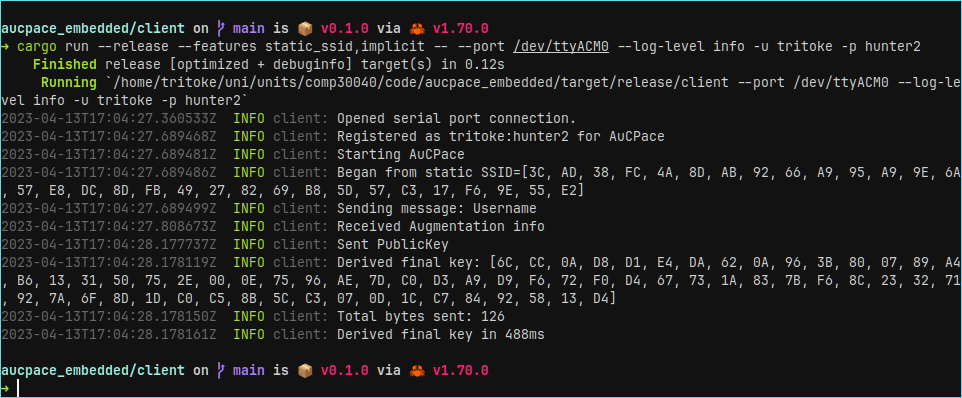
\includegraphics[width=\linewidth]{aucpace_embedded_client.png}
  \caption{AuCPace Embedded Client Output}
  \label{fig:aucpace-embedded-client}
\end{figure}

\begin{figure}[H]
  \centering

  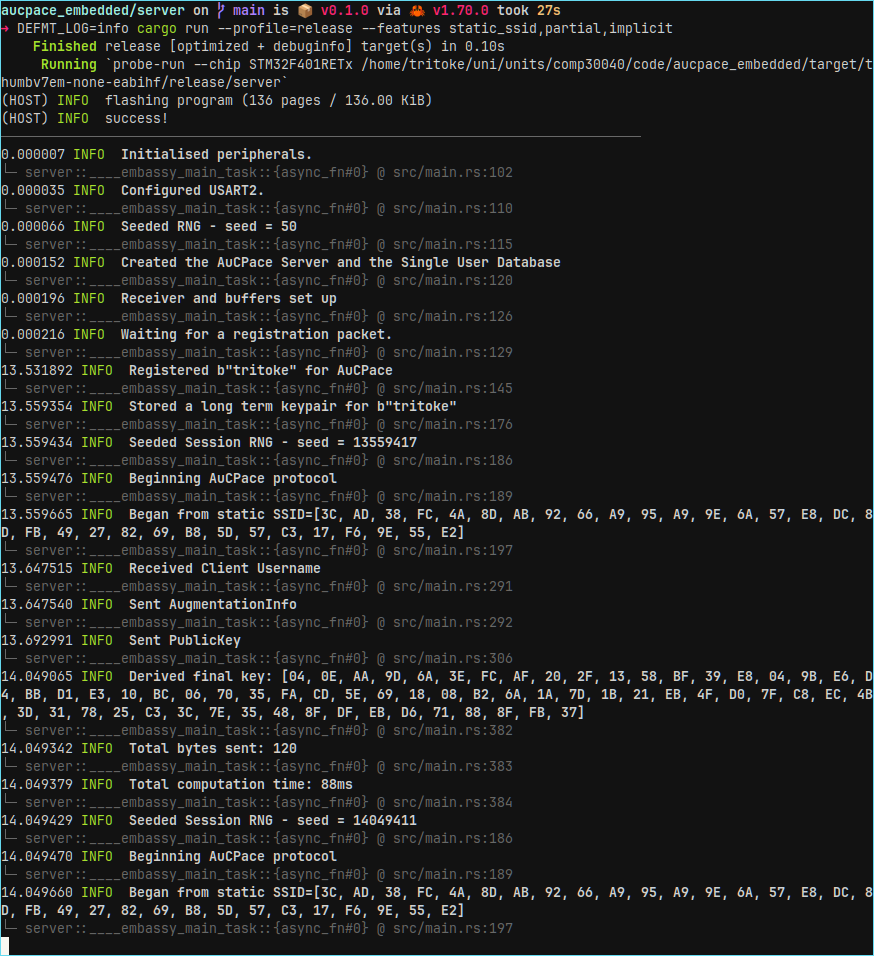
\includegraphics[width=\linewidth]{aucpace_embedded_server.png}
  \caption{AuCPace Embedded Server Output}
  \label{fig:aucpace-embedded-server}
\end{figure}

\begin{center}
  \rowcolors{0}{}{mintbg}
  \captionof{table}{Code size and Compute time by feature flag with \texttt{profile=server}}
  \label{tab:aucpace-embedded-benchmarks-server}
  \begin{tabular}{ ccccc }
    \toprule
    \texttt{strong} & \texttt{implicit} & \texttt{partial} & code size (Kib) & Compute time (ms) \\
    \midrule
    \xmark & \xmark & \xmark & 82 & 169 \\
    \xmark & \xmark & \cmark & 83 & 139 \\
    \xmark & \cmark & \xmark & 83 & 135 \\
    \xmark & \cmark & \cmark & 83 & 103 \\
    \cmark & \xmark & \xmark & 88 & 171 \\
    \cmark & \xmark & \cmark & 88 & 138 \\
    \cmark & \cmark & \xmark & 87 & 134 \\
    \cmark & \cmark & \cmark & 88 & 103 \\
    \bottomrule
  \end{tabular}
\end{center}

\begin{center}
  \rowcolors{0}{}{mintbg}
  \captionof{table}{Code size and Compute time by feature flag with \texttt{profile=server} and a static SSID}
  \label{tab:aucpace-embedded-benchmarks-server-static}
  \begin{tabular}{ ccccc }
    \toprule
    \texttt{strong} & \texttt{implicit} & \texttt{partial} & code size (Kib) & Compute time (ms) \\
    \midrule
    \xmark & \xmark & \xmark & 81 & 169 \\
    \xmark & \xmark & \cmark & 82 & 139 \\
    \xmark & \cmark & \xmark & 82 & 134 \\
    \xmark & \cmark & \cmark & 82 & 103 \\
    \cmark & \xmark & \xmark & 86 & 171 \\
    \cmark & \xmark & \cmark & 87 & 139 \\
    \cmark & \cmark & \xmark & 87 & 135 \\
    \cmark & \cmark & \cmark & 87 & 102 \\
    \bottomrule
  \end{tabular}
\end{center}

\begin{center}
  \rowcolors{0}{}{mintbg}
  \captionof{table}{Code size and Compute time by feature flag with \texttt{profile=release}}
  \label{tab:aucpace-embedded-benchmarks-release}
  \begin{tabular}{ ccccc }
    \toprule
    \texttt{strong} & \texttt{implicit} & \texttt{partial} & code size (Kib) & Compute time (ms) \\
    \midrule
    \xmark & \xmark & \xmark & 131 & 148 \\
    \xmark & \xmark & \cmark & 136 & 121 \\
    \xmark & \cmark & \xmark & 131 & 117 \\
    \xmark & \cmark & \cmark & 137 & 89 \\
    \cmark & \xmark & \xmark & 138 & 148 \\
    \cmark & \xmark & \cmark & 141 & 118 \\
    \cmark & \cmark & \xmark & 138 & 117 \\
    \cmark & \cmark & \cmark & 141 & 89 \\
    \bottomrule
  \end{tabular}
\end{center}

\begin{center}
  \rowcolors{0}{}{mintbg}
  \captionof{table}{Code size and Compute time by feature flag with \texttt{profile=release} and a static SSID}
  \label{tab:aucpace-embedded-benchmarks-release-static}
  \begin{tabular}{ ccccc }
    \toprule
    \texttt{strong} & \texttt{implicit} & \texttt{partial} & code size (Kib) & Compute time (ms) \\
    \midrule
    \xmark & \xmark & \xmark & 130 & 145 \\
    \xmark & \xmark & \cmark & 135 & 119 \\
    \xmark & \cmark & \xmark & 131 & 115 \\
    \xmark & \cmark & \cmark & 136 & 88 \\
    \cmark & \xmark & \xmark & 137 & 146 \\
    \cmark & \xmark & \cmark & 140 & 120 \\
    \cmark & \cmark & \xmark & 137 & 117 \\
    \cmark & \cmark & \cmark & 141 & 89 \\
    \bottomrule
  \end{tabular}
\end{center}

\begin{figure}[H]
  \centering
  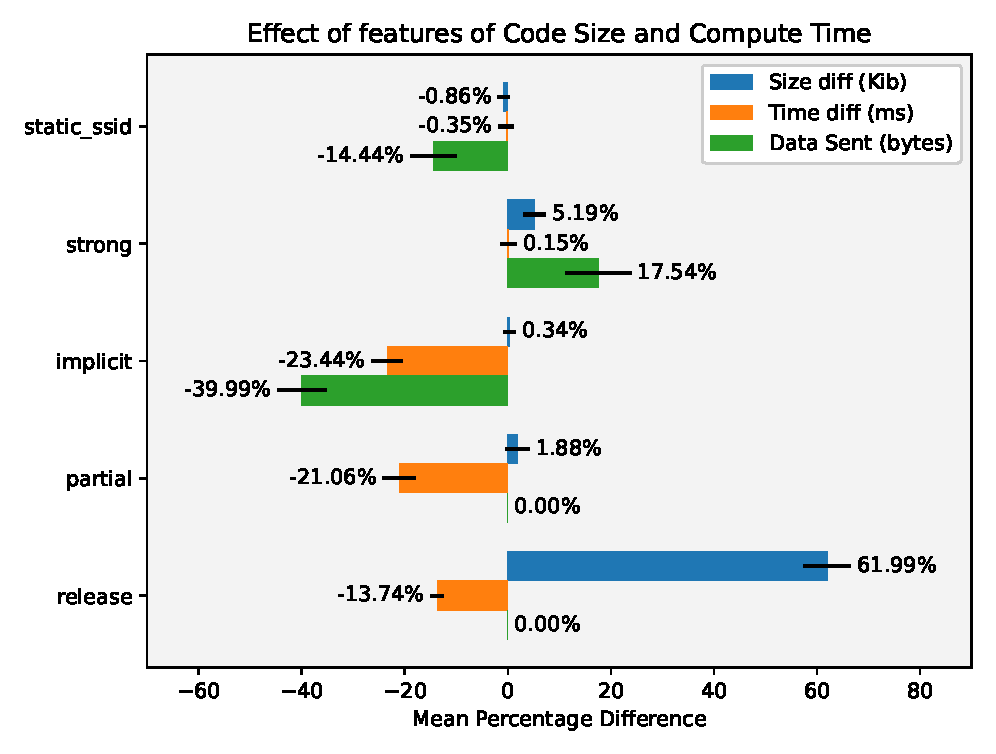
\includegraphics{assets/feature_effects.eps}
  \caption{Plot of the effect of different feature flags and compiler modes}
\end{figure}

\clearpage

\section{Breaking everything}
By happenstance I was reading NCC Group's recent review of Whatsapp's \texttt{opaque-ke} crate \cite{whatsapp-are-dumb-too, whatsapp-are-dumb-too-report}.
While reading the report the following finding caught my eye:
\begin{figure}[H]
  \centering

  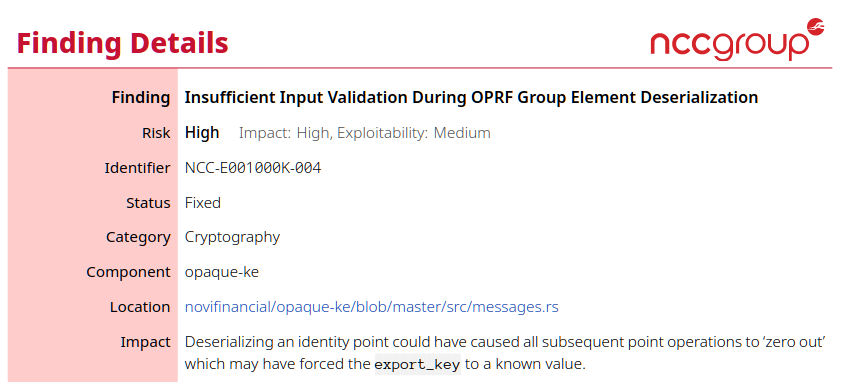
\includegraphics[width=\linewidth]{high_finding.png}
  \caption{High severity finding from \cite{whatsapp-are-dumb-too-report}.}
  \label{fig:high-severity-finding}
\end{figure}

In Whatsapp's implementation of OPAQUE \cite{opaque}, they used the \texttt{RistrettoPoint} type from \texttt{curve25519-dalek}, and while deserialising this type they didn't have any checks to see if this point was the identity point.
\Citeauthor{whatsapp-are-dumb-too-report} point out that this leads all subsequent point operations to "zero out" and thus cause the shared key to have a known value.
Unsure of whether this would also break my \gls{aucpace} implementation I modified \texttt{key\_agreement.rs} to have the client act as a malicious adversary and to send this identity point.

\rustcode{Malicious AuCPace Client}{assets/neutral_point_send.rs}

\begin{figure}[H]
  \centering

  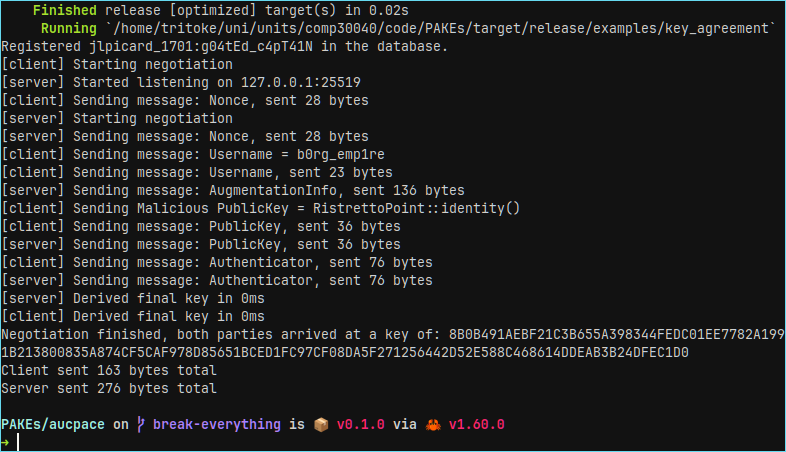
\includegraphics[width=\linewidth]{malicious_aucpace.png}
  \caption{Malicious AuCPace Client}
  \label{fig:break-everything}
\end{figure}

To my dismay it worked.
I immediately imformed RustCrypto of the problem and started working on a fix.

\subsection{Identifying the extent of the damage}
So what could a malicious attacker do with this bug?

\begin{itemize}
  \item{Impersonate any user, even a user who has never registered, even when no user has ever registered.}
  \item{Impersonate any server, to any user, regardless of whether they've registered with the server.}
\end{itemize}

Safe to say this is about as bad as it gets.

\subsection{Fixing the problem}
Thankfully the fix for this issue is incredibly simple.
The \gls{aucpace} protocol specifies points at which to abort the protocol should an invalid point is encountered.
Thus everywhere \gls{aucpace} says to abort if the point is invalid, we put in a check for the identity point.

\codediff[minted options={firstline=575, lastline=589}]{Patch for checking the identity element.}{assets/fix.diff}

It is clear to see that this is a very simple patch the main issue is ensuring it is caught everywhere.

\subsection{Why was this not caught earlier?}
There are several reasons why this wasn't caught earlier:
\begin{enumerate}
  \item{My lack of familiarity with \gls{ecc} -- this was my first time ever using \gls{ecc} and it was simply not something I knew to look out for.}
  \item{My decisiion to implement based on the paper not the \gls{ietf} document -- the paper mentions only to abort if a point is invalid. However there are two ways a point can be invalid, it can be off the curve, and it can be the identity point. \texttt{curve25519-dalek} makes the former unrepresentable using Rust's type system, hence my belief that this check was unnecessary. However the \gls{ietf} draft of \gls{aucpace} mentions explicitly to check for the identity element \cite{ietf-aucpace}.}
  \item{This is quite a subtle bug -- it is hard to spot when you are unfamiliar with \gls{ecc}, case and point Whatsapp made this mistake as well, and so did the the core developers of Java. Java's CVE-2022-21449 "Psychic Signatures" \cite{java-psychic-signatures}, had the same bug in their implementation of \gls{ecdsa}. Introduced in commit \texttt{3c12c4b0f35} Dec 2018 fixed in \texttt{e2f8ce9c3ff} Jan 2022, all in it took 3 years for this same bug to get found and patched in Java.}
\end{enumerate}

\subsection{How to prevent this bug from ever happening again}
Two changes have been implemented to prevent this bug from ever happening again:
\begin{enumerate}
  \item{Every method that handles a RistrettoPoint from the network checks it to make sure it is not the identity point.}
  \item{There are now tests for every method of both the Client and Server to ensure that providing an invalid point returns an \texttt{IllegalPointError}.}
\end{enumerate}

There is a better way to fix this however, RustCrypto's \texttt{elliptic-curve} module solves this problem using the power of Rust's type system.
They have a \texttt{NonIdentity} type which is guaranteed to never be the identity element.
When Curve25519 is introduced to \texttt{elliptic-curve} the library will be refactored to move over to this type.



% print the glossary
\printnoidxglossaries{}

% this determines the style in which
% the references are printed, other
% possible values are plain and abbrv
\bibliographystyle{plain}       
\nocite{*}
\bibliography{refs}

%% Appendices start here
\appendix
\chapter{Python implementation of EKE}

While researching Bellovin and Merritt's EKE scheme\cite{eke}, I created a full implementation of the scheme in Python.
The full code can be found at \url{https://github.com/tritoke/eke_python}.
The core negotiation functions for the client and server have been included below:

\pythoncode[minted options={firstline=36,lastline=76,gobble=4}]{Client Negotiate}{eke_python/client.py}
\pythoncode[minted options={firstline=50,lastline=81,gobble=4}]{Server Negotiate}{eke_python/server.py}


\chapter{Python implementation of SRP}
\label{chap:appendix-srp}

While conducting my initial research on PAKEs I came across \gls{srp}\cite{srp}.
\gls{srp} is the first protocol I looked at which took the approach of encoding values as \gls{dh} group elements.
To understand this approach better I chose to create a toy implementation.
The full code can be found at \url{https://github.com/tritoke/srp_python}.
The core negotiation functions for the client and server have been included below:

\pythoncode[minted options={firstline=37,lastline=72}]{Client Negotiate}{srp_python/client.py}
\pythoncode[minted options={firstline=57,lastline=115}]{Server Negotiate}{srp_python/server.py}



\end{document}
